\chapter{Information Loss Measures for Geo-Referenced Data} \label{sec:util}
\chaptermark{Information Loss Measures}

When an SDC method is applied to reduce the risks shown in Chapter \ref{sec:risk}, invariably some spatial aggregates may need to be altered, coarsened, or otherwise changed, leading to a loss of information compared to unprotected data. This chapter discusses how to assess such information loss, while keeping in mind the specific spatial character of the data.

\section{Measures of distributional distance} \label{sec:util_DD}

A grid map of frequency counts can be interpreted as a two-dimensional frequency distribution, visualised as a spatial histogram. Distortion of such a distribution can be measured by distance metrics between the original, unprotected map and the protected map.

\subsection{Hellinger Distance, Mean Squared Error, Mean Absolute Error} \label{sec:util_DD_hd}

The Hellinger Distance (HD) is an information-theoretical distance measure between two distributions. Its use in assessing the information loss after tabular data protection is well established, see e.g. \cite{ShlomoEtAl2015}, \cite{AntalEtAl2017}, \cite{ShlomoYoung2006} as well as \citet[4.7.2]{HundepoolEtAl2024}. An application to grid maps is described in \cite{GussenbauerEtAl2023}.

Formally, let us number the cells in the grid by $j = 1, \dots, M$. The original cell-level aggregates $X_j$ are compared to the aggregates after protection, which we call $X'_j$.
The Hellinger distance is defined as
\begin{equation} \label{eq:util_hd}
\mathrm{HD}\,(X, X') = \frac{1}{\sqrt{2}} \sqrt{\sum_{j=1}^M \left (\sqrt{X'_j} - \sqrt{X_j} \right )^2}.
\end{equation}

If $X_j$ and $X'_j$ are counts, the Hellinger distance is between 0 and $\sqrt{N}$, where $N$ is the sum of counts over the whole map \citep{ShlomoEtAl2015}.\footnote{
    This holds whenever the SDC mechanism does not change the total sum of counts $N$. For rounding-based or noise-based methods (like CKM; see section \ref{sec:ckm}) this may not be so. In that case the Hellinger distance is between 0 and the more general upper bound $\sqrt{N' + N} / \sqrt{2}$ (where $N'$ is the total sum of altered counts over the map).
} Alternatively, both $X$ and $X'$ can be re-scaled to the form of a discrete probability distribution, such that $X_j$ and $X'_j$ each sum to 1. In that case $\mathrm{HD} \in [0 \,, 1]$.
In any case a Hellinger distance of 0 signifies no information loss.

\subsubsection{Comparing HD and MSE / MAE}

The Hellinger distance may be contrasted with two other prevailing measures. The Mean squared error (MSE) and Mean absolute error (MAE) are common descriptive statistics that can be given a distance interpretation.
Formally, they are defined as follows:
\begin{equation} \label{eq:util_mse}
\mathrm{MSE}\,(X, X') = \frac{1}{M} \sum_{j=1}^M \left(X'_j - X_j\right)^2
\end{equation}
\begin{equation} \label{eq:util_mae}
\mathrm{MAE}\,(X, X') = \frac{1}{M} \sum_{j=1}^M \left| X'_j - X_j \right|.
\end{equation}

When choosing a measure for comparison, data suppliers should consider the following principle:
\textit{A distance measure between (spatial) distributions is useful, when an increase in distance is indicative of a deterioration of the perturbed map in comparison to the original.}\\

\begin{tcolorbox}[breakable]
\emph{Example}:
Consider the following simplified distribution of counts over a 4 $\times$ 4 grid map:
\[ 
\mathbf{X} = \begin{matrix} 
0 & 0 & 0 & 0 \\
0 & 4 & 1 & 0 \\
0 & 4 & 1 & 0 \\
0 & 0 & 0 & 0 \\
\end{matrix}
\]
We will compare this distribution with two ``perturbed" maps, labelled $\mathbf{X}'_{(1)}$ and $\mathbf{X}'_{(2)}$ respectively:
\[
\mathbf{X}'_{(1)} =
\begin{matrix} 
1 & 1 & 1 & 1 \\
1 & 0 & 0 & 1 \\
1 & 0 & 0 & 1 \\
1 & 0 & 0 & 1 \\
\end{matrix}\hspace{1cm}
\mathbf{X}'_{(2)} =
\begin{matrix} 
0 & 0  & 0 & 0 \\
0 & 0  & 0 & 0 \\
0 & 10 & 0 & 0 \\
0 & 0  & 0 & 0 \\
\end{matrix} 
\]
Results for MSE, MAE and HD are shown in Table \ref{tab:util_hd_mae_mse}.
The Hellinger distance has the property that it reaches its theoretical maximum when the underlying distributions have \textit{disjoint spatial support}. Practically speaking, this means that all previously inhabited areas would be uninhabited, arguably a \emph{worst case} for mapping. This is shown in $\mathbf{X}'_{(1)}$.

On the other hand, $\mathbf{X}'_{(2)}$ exemplifies an aggregation of the populated part of $\mathbf{X}$ (symbolizing a town, village or similar) to a smaller sub-area within. While this may be a grave error, it is arguably less so than the one shown in $\mathbf{X}'_{(1)}$. 
Looking at Table \ref{tab:util_hd_mae_mse}, we find that comparing the original $\mathbf{X}$ to $\mathbf{X}'_{(1)}$ yields the maximum Hellinger distance. The MSE, however, is lower when comparing $\mathbf{X}$ to $\mathbf{X}'_{(1)}$ than when comparing to $\mathbf{X}'_{(2)}$. The Hellinger distance is here more in line with the assumed rationale of the map maker.\footnote{
    It is granted that such extreme deviations as $\mathbf{X}'_{(1)}$ are unlikely to occur in practice. Nevertheless, populating at least some unpopulated cells is a common feature of several spatial SDC mechanisms, and it is good practice to consider what kind of data distortion would constitute a worst case.}\\

Another property of the Hellinger distance is of interest when comparing spatial distributions. To display it, consider two more perturbations of $\mathbf{X}$, labelled $\mathbf{X}'_{(3)}$ and $\mathbf{X}'_{(4)}$ shown below. Both maps differ from $\mathbf{X}$ by having one tenth of the distribution mass shifted between neighboring grid cells.
\[
\mathbf{X}'_{(3)} =
\begin{matrix} 
0 & 0 & 0 & 0 \\
0 & 5 & 1 & 0 \\
0 & 3 & 1 & 0 \\
0 & 0 & 0 & 0 \\
\end{matrix} \hspace{1cm}
\mathbf{X}'_{(4)} =
\begin{matrix} 
0 & 0 & 0 & 0 \\
0 & 4 & 2 & 0 \\
0 & 4 & 0 & 0 \\
0 & 0 & 0 & 0 \\
\end{matrix}
\]
Again, distance measures are shown in Table \ref{tab:util_hd_mae_mse}. It can be seen that MSE and MAE do not distinguish between $\mathbf{X}'_{(3)}$ and $\mathbf{X}'_{(4)}$. For mapping purposes however, shifting mass between two high-population areas $(\mathbf{X}'_{(3)})$ may be seen as a smaller error than doubling the population in one area and depopulating another $(\mathbf{X}'_{(4)})$. This rationale is covered by the Hellinger distance, but not by MSE and MAE.\footnote{
    This is because HD sums squared deviations of square roots, which penalizes large \emph{relative} changes \citep{AntalEtAl2017}, while MSE and MAE depend on \emph{absolute} changes.}

\begin{table}[H]
    \centering
    \begin{tabular}{c | c c c | c c c |}
            \multirow{2}{*}{$\mathbf{X}$ vs. }& \multicolumn{3}{c}{count} & \multicolumn{3}{c}{scaled} \\
               & MSE & MAE & HD & MSE & MAE & HD \\
        \hline
    $\mathbf{X}'_{(1)}$ & 2.75 & 1.25 & 3.16 & 0.028 & 0.125 & 1.000 \\
    $\mathbf{X}'_{(2)}$ & 3.38 & 0.75 & 1.92 & 0.033 & 0.075 & 0.606 \\
    $\mathbf{X}'_{(3)}$ & 0.13 & 0.13 & 0.25 & 0.001 & 0.013 & 0.080 \\
    $\mathbf{X}'_{(4)}$ & 0.13 & 0.13 & 0.77 & 0.001 & 0.013 & 0.242 \\
        \hline
    \end{tabular}
    \caption{Distributional distances between maps $\mathbf{X}$ vs. $\mathbf{X}'_{(1)}, \dots, \mathbf{X}'_{(4)}$}
    \label{tab:util_hd_mae_mse}
\end{table}
\end{tcolorbox}


\subsection{Earth Mover distance / Wasserstein distance} \label{sec:util_DD_kwd}

The Earth Mover distance, also known as \emph{Kantorovich-Wasserstein distance} (KWD), or simply Wasserstein distance, is a distance measure between distributions applicable to spatial histograms. While it is more demanding to compute than the metrics from \ref{sec:util_DD_hd}, it offers some theoretical advantages. 
We begin by showing a limitation of the HD, MSE, and MAE metrics introduced above.

\begin{tcolorbox}[breakable]
\emph{Example}:
Consider the following case of a (very much simplified) count distribution in a 4 $\times$ 4 grid map. The example is adapted from \cite{GussenbauerEtAl2023} and \cite{RicciatoGualandi2024}. 10 population units are spread over 5 grid cells, symbolizing a small spatial cluster:
\[
\mathbf{X} = \begin{matrix} 0 & 2 & 0 & 0 \\
                  2 & 2 & 2 & 0 \\
                  0 & 2 & 0 & 0 \\
                  0 & 0 & 0 & 0 \end{matrix}
\]
We now offer four hypothetical perturbations, shown as $\mathbf{X}'_{(1)}, \dots, \mathbf{X}'_{(4)}$ below. Loosely, the first two $(\mathbf{X}'_{(1)} \text{ and } \mathbf{X}'_{(2)})$ correspond to shifting some units around in space, whereas the latter two $(\mathbf{X}'_{(3)} \text{ and } \mathbf{X}'_{(4)})$ are different local aggregations.
\begin{align*}
\mathbf{X}'_{(1)} = \begin{matrix} 0 & 0  & 2 & 0 \\
                          2 & 2  & 2 & 0 \\
                          2 & 0  & 0 & 0 \\
                          0 & 0  & 0 & 0 \end{matrix} & \hspace{1cm}
\mathbf{X}'_{(2)} = \begin{matrix} 0 & 0  & 0 & 2 \\
                          2 & 2  & 2 & 0 \\
                          0 & 0  & 0 & 0 \\
                          0 & 0  & 0 & 2 \end{matrix} \\ & \\
\mathbf{X}'_{(3)} = \begin{matrix} 0 & 0  & 0  & 0 \\
                          0 & 10 & 0  & 0 \\
                          0 & 0  & 0  & 0 \\
                          0 & 0  & 0  & 0 \end{matrix} & \hspace{1cm}
\mathbf{X}'_{(4)} = \begin{matrix} 0 & 0  & 0  & 0 \\
                          0 & 0  & 10 & 0 \\
                          0 & 0  & 0  & 0 \\
                          0 & 0  & 0  & 0 \end{matrix}
\end{align*}
Most data suppliers would judge $\mathbf{X}'_{(2)}$ inferior to $\mathbf{X}'_{(1)}$, since the former shifts units \emph{further away} than the latter, compared to the true distribution $\mathbf{X}$. Similarly, in $\mathbf{X}'_{(3)}$ and $\mathbf{X}'_{(4)}$, while the information loss from aggregation is the same, the latter also shifts the \emph{geometrical center} of the distribution, while the former keeps it.
It would thus be reasonable to demand a distance measure which gives us $\mathrm{Dist.}(\mathbf{X}, \mathbf{X}'_{(2)}) > \mathrm{Dist.}(\mathbf{X}, \mathbf{X}'_{(1)})$ and $\mathrm{Dist.}(\mathbf{X}, \mathbf{X}'_{(4)}) > \mathrm{Dist.}(\mathbf{X}, \mathbf{X}'_{(3)})$.\footnote{
    Recall our principle stated above: \textit{a distance measure is useful insofar as an inferior map is associated with a larger distance}.}
    
Actual distributional distances are given in Table \ref{tab:util_nokwd}. 
For any given measure introduced so far we get $\mathrm{Dist.}(\mathbf{X}, \mathbf{X}'_{(2)}) = \mathrm{Dist.}(\mathbf{X}, \mathbf{X}'_{(1)})$ and $\mathrm{Dist.}(\mathbf{X}, \mathbf{X}'_{(4)}) = \mathrm{Dist.}(\mathbf{X}, \mathbf{X}'_{(3)})$. In other words, these metrics are not discriminating quite as we would want them to.\footnote{
    The reason is that changes in mere \emph{position} are not taken into account.}

\begin{table}[H]
    \centering
    \begin{tabular}{c | c c c |}
    $\mathbf{X}$ vs. & MSE & MAE & HD \\
    \hline
    $\mathbf{X}'_{(1)}$ & 1.00 & 0.50 & 2.00 \\
    $\mathbf{X}'_{(2)}$ & 1.00 & 0.50 & 2.00 \\
    \hline
    $\mathbf{X}'_{(3)}$ & 5.00 & 1.00 & 2.35 \\
    $\mathbf{X}'_{(4)}$ & 5.00 & 1.00 & 2.35 \\
        \hline
    \end{tabular}
    \caption{MSE, MAE, and HD between maps $\mathbf{X}$ vs. $\mathbf{X}'_{(1)}, \dots, \mathbf{X}'_{(4)}$}
    \label{tab:util_nokwd}
\end{table}
\end{tcolorbox}

Generally speaking, such concepts as `further away' and `shifted geometrical center' are not covered by the distributional distances of section \ref{sec:util_DD_hd}. They do not explicitly take the \emph{spatial dimension of error} into account. The Kantorovich-Wasserstein distance (KWD), on the other hand, does this, by conceptualizing the distance between distributions as a problem of \emph{optimal transport}.
The idea is to transform one distribution, say the perturbed $X'$, into the other, say the original $X$, by transporting units (or, more generally: distribution mass) around the map, until both distributions look alike. Each act of transportation is evaluated at `costs' equivalent to the geographical distance covered.
%\footnote{
    %Shifting 2 units by 3 cells to the left 'costs' $2 \cdot 3 = 6$, etc. We consider here for the geographical distance the Euclidean, or straight-line distance, but KWD generalizes to others, such as the Manhattan distance. Units that do not need to be moved are evaluated at zero 'costs'.}
KWD is defined as the total cost of the `cheapest' way to perform such a transformation.

Formally, computing KWD involves solving the following optimization problem. We denote the shifted distribution mass (e.g. a certain number of population units) between grid cell $j$ and $k$ by $\Delta X_{jk}$. The (spatial) distance between these grid cells is $d_{jk}$. We then need to solve:
\begin{equation} \label{eq:util_kwd}
\begin{aligned}
    & \mathrm{KWD}\,(X, X') = & \underset{\Delta X_{jk}}{\text{min}} \quad & \frac{1}{N} \sum_{j=1}^M \sum_{k=1}^M \Delta X_{jk} \cdot d_{jk} & \\
    & & \text{s.t.} \quad & \sum_{k=1}^M \Delta X_{jk} = X_j & \forall j = 1, \dots, M\\
    & & & \sum_{j=1}^M \Delta X_{jk} = X'_k & \forall k = 1, \dots, M \\
    & & & \Delta X_{jk} \geq 0 & \forall j,k = 1, \dots, M.
\end{aligned}
\end{equation}

\begin{tcolorbox}[breakable]
\emph{Example cont'd:}
Going back to our example, we find that transforming $\mathbf{X}'_{(1)}$ back to $\mathbf{X}$ is most efficiently achieved by conceptually shifting the 2 units in the first row one cell to the left, the 2 units in the third row one cell to the right. This is associated with a combined `cost' of $2 \cdot 1 + 2 \cdot 1 = 4$, hence $\mathrm{KWD}(\mathbf{X}, \mathbf{X}'_{(1)}) = 4/10 = 0.4$. The optimal transport plan for $\mathbf{X}'_{(2)}$ gives us $2 \cdot 2 + 2 \cdot \sqrt{1^2 + 2^2} \approx 8.47$, therefore $\mathrm{KWD}(\mathbf{X}, \mathbf{X}'_{(2)}) \approx 0.85$.\footnote{
    By analogous reasoning we can find out that $\mathrm{KWD}(\mathbf{X}, \mathbf{X}'_{(4)}) > \mathrm{KWD}(\mathbf{X}, \mathbf{X}'_{(3)})$.}
In other words, the KWD discriminates in line with the assumed judgment of the data supplier, where (in this case) MSE, MAE, and HD did not.
\end{tcolorbox}

\subsubsection{Practical issues}

Computing KWD in practice requires a solver for the optimization procedure, as problems are not as simple as in the motivating example. When the number of bins in the spatial histogram is large, an exact solution may not be feasible computationally. \cite{BassettiEtAl2020} provide a method to approximate KWD in these cases. A ready-to-use implementation for the R software is the \texttt{SpatialKWD} package.
An example use for comparing spatial histograms by KWD is given in \cite{RicciatoColuccia2023}. An application specifically for assessing the impact of SDC is \cite{GussenbauerEtAl2023}.


\section{Measures of spatial association} \label{sec:util_SPAT}

\subsection{Variance-Mean ratio}

The Variance-Mean ratio (VMR) is a measure of dispersion. It can be used as a descriptive statistic to measure the overall level of spatial clustering in geo-referenced data \citep{Cressie1993}. Intuitively, if the distribution of population over a map is relatively homogeneous, then cell counts everywhere will not differ much from the average cell count. If, on the other hand, population is concentrated at one or a few points of the map and thin between, a high variance of counts results. By comparing the VMR before and after disclosure control, a first indication is given as to how the level of clustering is impacted.\footnote{
    Note: If the total number of population units in the map is not changed by SDC, then the mean too will stay the same and comparing VMR reduces to comparing the variance of the count distribution.} 

Formally, the VMR is measured as
\begin{equation}
    \mathrm{VMR}\,(X) = \frac{\frac{1}{M}\sum_{j = 1}^M (X_j - \bar{X})^2}{\bar{X}} = \frac{\mathrm{Var}(X)}{\mathrm{Mean}(X)}.
\end{equation}

The difference $\mathrm{VMR}\,(X') - \mathrm{VMR}\,(X)$ is positive if SDC has increased the level of spatial clustering, negative if it has decreased it.\\

If there exist only very few outliers and their impact on total dispersion is expected to be reduced then instead of $\mathrm{VMR}$ one can use its positional counterpart, i.e. MedAD-Median ratio, given as:

\begin{equation}
    \mathrm{MMR}\,(X) = \frac{\mathrm{MedAD}(X)}{\mathrm{Med}(X)},
\label{MMR}
\end{equation}
where $\mathrm{MedAD}(X)=\mathrm{Med}_{j=1,2,\ldots,M}|X_j-\mathrm{Med}(X)|$ is the Median Absolute Deviation of $X$. The interpretation of the difference $\mathrm{MMR}\,(X') - \mathrm{MMR}\,(X)$ is the same as $\mathrm{VMR}\,(X') - \mathrm{VMR}\,(X)$. The main limitation of (\ref{MMR}) is that when most cell counts are zero (in sparse grid data, for instance), it cannot be computed. Hence, MMR is useful only for such grids, where all (or almost all) data are non-zero.

On the other hand, one could be afraid that the double-use of the median (median absolute deviation from the median) in (\ref{MMR}) is somewhat `too robust'. That is, one can get the same MMR, even though the map has changed, which would not be informative.
To reduce the latter inconvenience, one can suggest also two alternative approaches. Firstly, the MedADM-Med ratio:
\begin{equation}
    \mathrm{MMR^*}\,(X) = \frac{\mathrm{MedADM}(X)}{\mathrm{Med}(X)},
\label{MMRx}
\end{equation}
where $\mathrm{MedADM}(X)=\mathrm{Med}_{j=1,2,\ldots,M}|X_j-\bar{X}|$ is the median absolute deviation from the mean. Secondly, the MeanAD-Med ratio:
\begin{equation}
    \mathrm{MMR^{**}}\,(X) = \frac{\mathrm{MeanAD}(X)}{\mathrm{Med}(X)},
\label{MMRxx}
\end{equation}
where 
%$\mathrm{MeanAD}(X)=\frac{\sum_{j=1}^M{|X_j-\mathrm{Med}(X)|}}{M}$. 
$\mathrm{MeanAD}(X)= \frac{1}{M} \sum_{j=1}^M |X_j-\mathrm{Med}(X)|$ is the mean absolute deviation from the median.
However, the problematic case of $\mathrm{Med}(X) = 0$ still exists both in (\ref{MMRx}) and in (\ref{MMRxx}). One can try to overcome it by assuming instead of a ``pure" median in (\ref{MMR}), (\ref{MMRx}) and (\ref{MMRxx}) the corrected median defined as follows:
\begin{equation}
\mathrm{\widetilde{med}}(X)=\mathrm{med}(X)+\frac{\mathop{\min}\limits_{j:X_{j}\ne 0}{|X_{j}|}}{M}.
\label{MEDc}
\end{equation}

\begin{tcolorbox}[breakable]
\emph{Example}:
$\mathbf{X}$ below shows a $6 \times 6$ grid map with original counts. $\mathbf{X}'$, to its right, shows a protected version. We want to calculate VMR and MMR.
\[ 
\mathbf{X} = \begin{matrix} 
2 & 4 & 0 & 0 & 0 & 0\\
4 & 2 & 0 & 0 & 0 & 0\\
0 & 0 & 2 & 3 & 2 & 0\\
0 & 0 & 0 & 5 & 4 & 1\\
0 & 0 & 3 & 4 & 2 & 0\\
0 & 0 & 0 & 4 & 0 & 2\\
\end{matrix}
\hspace{1cm}
\mathbf{X}' = \begin{matrix} 
3 & 3 & 0 & 0 & 0 & 0\\
3 & 3 & 0 & 0 & 0 & 0\\
0 & 0 & 2 & 2 & 2 & 2\\
0 & 0 & 2 & 2 & 2 & 2\\
0 & 0 & 2 & 2 & 2 & 2\\
0 & 0 & 2 & 2 & 2 & 2\\
\end{matrix}
\]
The sum of counts is 44 in both maps; hence the mean is $44/36 \approx 1.22$. For the variance we get 2.69 (left) and 1.32 (right) respectively. This gives us for the change in VMR:
\[
\mathrm{VMR}(\mathbf{X}') - \mathrm{VMR}(\mathbf{X})
= \frac{1.32}{1.22} - \frac{2.69}{1.22} \approx - 1.12.
\]
Because $\mathrm{med}(\mathbf{X})=0$, we cannot use directly measures (\ref{MMR}), (\ref{MMRx}) and (\ref{MMRxx}). However, we can use (\ref{MEDc}) and obtain $\mathrm{\widetilde{med}}(\mathbf{X})=0,028$ and $\mathrm{\widetilde{med}}(\mathbf{X}')=2,056$. Hence, $\mathrm{MedAD}(\mathbf{X}')=0.944$, $\mathrm{MedAD}(\mathbf{X})=0.028$, $\mathrm{MedADM}(\mathbf{X}')=1.222$, $\mathrm{MedADM}(\mathbf{X})=1.222$, $\mathrm{MeanAD}(\mathbf{X}')=1.043$, $\mathrm{MeanAD}(\mathbf{X})=1.227$ and in consequence,   the corrected measures are as follows 
\[
\mathrm{MMR}(\mathbf{X}') - \mathrm{MMR}(\mathbf{X})
= \frac{0.944}{2.056} - \frac{0.028}{0.028} \approx -0.541,
\]
\[
\mathrm{MMR^*}(\mathbf{X}') - \mathrm{MMR^*}(\mathbf{X})
= \frac{1.222}{2.056} - \frac{1.222}{0.028}\approx -43.405,
\]
and
\[
\mathrm{MMR^{**}}(\mathbf{X}') - \mathrm{MMR^{**}}(\mathbf{X})
= \frac{1.043}{2.056} - \frac{1.227}{0.028}\approx -43.659.
\]

This means the protected map has a markedly lower level of clustering compared to the original. However, the two last measures seem to slightly overestimate the information loss. 
\end{tcolorbox}


\subsection{Moran's $\mathcal{I}$} \label{sec:util_moran}

% Moran plots as a graphical/visual way to compare original and perturbed autocorrelations ? What do you think ?
% I make a proposition a the end of the subsection

The \emph{Moran's $\mathcal{I}$ statistic}, proposed by \cite{Moran1950}, was conceived as a measure of spatial autocorrelation of spatial objects. In general, the global Moran's $\mathcal{I}$ statistic is of the form
\begin{equation}
    \mathcal{I}\stackrel{df}{=}\frac{n}{w}\frac{\sum_{i=1}^n{\sum_{j=1}^n{w_{ij}(x_i-\overline{x})(x_j-\overline{x})}}}{\sum_{i=1}^n{(x_i-\overline{x})^2}},
\label{globalI}
\end{equation}
where $n$ is the number of spatial units, $x_i$ is the value of the variable $X$ for $i$-th spatial unit, $\overline{x}$ is the mean of $X$ and $w_{ij}$ is the (non-negative) measure of closeness of $i$-th and $j$-th units with $w_{ii}=0$, ($i,j=1,2,\ldots,n$), $w=\sum_{i=1}^n{\sum_{j=1}^n{w_{ij}}}$.

Values of $\mathcal{I}$ belong usually to the interval $[-1,1]$.\footnote{If the matrix $\mathbf{W}=[w_{ij}],i,j=1,2,\ldots,n$ is symmetric and row--normalized.} Values significantly below $-1/(n-1)$ indicate negative spatial autocorrelation and values significantly above $-1/(n-1)$ indicate positive spatial autocorrelation. If $\mathcal{I}=-1$ then autocorrelation (dispersion) is perfect, if $\mathcal{I}=0$ then no autocorrelation occurs (i.e. we are dealing with perfect randomness). $\mathcal{I}=1$ indicates also perfect autocorrelation, but in the opposite direction.

In constructing (\ref{globalI}) the most important role seems to be played by the matrix of weights $\mathbf{W}=[w_{ij}]$, $i,j=1,2,\ldots,n$. It reflects the closeness of spatial units which can be defined in various ways. A classical approach in this context is based on physical neighbourhood, i.e. on existing common boundaries arbitrarily established (contiguity). More formally, two areas (e.g. grid tiles) are neighbours if they have a common frontier. Two approach in this respect are common: rook contiguity (when only common edges of polygons reflecting borders of given areas are considered to define the neighbor relation) or queen contiguity (when not only common edges but also common vertices are taken into account in this context). Due to better usefulness (e.g. for irregular polygons and reduction of possible inaccuracies) the use of queen criterion is recommended in practice. 

Alternatively, the neighbourhood can also be defined on the basis of a similarity of spatial units with regards to the distribution of a given composite social or economic phenomenon. The distance between given objects is here expressed by distance of vectors of values of relevant variables for them. Of course, they can include also some geographical information (e.g. country of birth), but it is not an absolute priority in this case. That is, it is assumed that such phenomenon is described by a number (say, $m$) variables. Each object is therefore described by a vector from $\mathbb{R}^m$. Using a relevant metric (e.g. Euclidean, city -- called also Manhattan, Minkowski, etc.) one can measure the distance between each pair of objects. The entries of matrix $\mathbf{W}$ can be simply such distances. Alternatively, $\mathbf{W}$ may be established in a binary way, i.e. as $w_{ij}=1$ (not neighbours) if $d_{ij}>q$ and $w_{ij}=0$ (neighbours) otherwise, where $d_{ij}$ is the distance between $i$-th and $j$-th objects and $q>0$ -- an arbitrarily established threshold. A more formal presentation and discussion on these topics was conducted by \cite{Mlodak2013}. The measures of information loss proposed in this paper were implemented to the \texttt{sdcMicro} R-package.   

It is worth noting that the variables describing the phenomenon being a base for identification of neighbourhood should be different than variables being perturbed in the SDC process (the neighbourhood is independent of the purpose of current analysis and cannot be perturbed). This means that only non-identifiers, non-quasi identifiers or non-sensitive variables can be used here.\\
%We could mention here the attention needed in choosing the matrix of weights (choosing contiguity or a distance, choosing a threshold beyond that the weights are set to zero, etc.) because it could have a substantial influence on the measure of the Moran I. Moreover, the matrix of weights has to be normalized, otherwise we create an heterogeinty between the units with a lot of neighbors and those with less. 
%(See \cite{BellefonEtAlt_2018})

An efficient measure of information loss due to global autocorrelation should satisfy the following expectations:
\begin{itemize}
    \item It should compare the loss of information of different SDC processes;
    \item it should be able to sort SDC processes in the right order w.r.t. distortion of spatial autocorrelation;
    \item it should clearly indicate the following situations, when they occur:
    \begin{itemize}
        \item a negative autocorrelation is weakened by the SDC process, 
        \item a positive autocorrelation is strengthened by the SDC process,
        \item a weak negative link is becoming a weak positive link by the SDC process;
    \end{itemize}
    \item it should provide information on the direction of the change (increase or decrease);
    \item it should be normalized on [-1,1].
\end{itemize}

It seems that these postulates are satisfied by the following measure:
\begin{equation}
\mathrm{ILM}\stackrel{df}{=}\frac{\mathcal{I}'-\mathcal{I}}{2},
\label{globalloss}
\end{equation}
where $\mathcal{I}'$ is the Moran's $\mathcal{I}$ global statistics (\ref{globalI}) after disclosure protection within the SDC process. The coefficient (\ref{globalloss}) takes value from $[-1,1]$ and hence can be presented in \%. If $\mathrm{ILM}=0$ then no loss is incurred, whereas $|\mathrm{ILM}|=1$ means the loss is maximal.%\\

\begin{tcolorbox}[breakable]
\emph{Example}:
Consider the following simplified distribution of counts over a 6 $\times$ 6 grid map, denoted by $\mathbf{X}$. Sensitive counts (considered here as any grid cell smaller than 5) are protected by two iterations of the quadtree mechanism (see section \ref{sec:quadtree}), yielding protected map $\mathbf{X}'$.

\[ 
\mathbf{X} = \begin{matrix} 
2 & 4 & 0 & 0 & 0 & 0\\
4 & 2 & 0 & 0 & 0 & 0\\
0 & 0 & 2 & 3 & 2 & 0\\
0 & 0 & 0 & 5 & 4 & 1\\
0 & 0 & 3 & 4 & 2 & 0\\
0 & 0 & 0 & 4 & 0 & 2\\
\end{matrix}
\hspace{1cm}
\mathbf{X}' = \begin{matrix} 
3 & 3 & 0 & 0 & 0 & 0\\
3 & 3 & 0 & 0 & 0 & 0\\
0 & 0 & 2 & 2 & 2 & 2\\
0 & 0 & 2 & 2 & 2 & 2\\
0 & 0 & 2 & 2 & 2 & 2\\
0 & 0 & 2 & 2 & 2 & 2\\
\end{matrix}
\]

We aim to measure Moran's $\mathcal{I}$, using as our criterion for neighbourhood the `queen'-contiguity (in other words, a grid cell is neighbour to the 8 cells surrounding it, including diagonally). With $6^2 = 36$ cells, the weight matrix $\mathbf{W}$ has 36 rows and 36 columns. The first row encodes all neighbors of the first cell ($i = 1$), of which there are three: directly east ($j = 2$), directly south ($j = 7$) and diagonally southeast ($j = 8$) -- most cells will have more neighbors, because they don't lie at a corner. For the first row of weights $w_{1j}$ we thus get
\[
w_{1j} = 1 \text{ for } j = 2,7,8 \text{ and } w_{1j} = 0 \text{ else}.
\]
To avoid the distorting effect of a differing number of neighbours between cells, we row-standardize to
\[
w_{1j} = \frac{1}{3} \text{ for } j = 2,7,8 \text{ and } w_{1j} = 0 \text{ else}
\]
so that $\sum_j w_{1j} = 1$. For all other rows we proceed likewise.\footnote{
    The creation of a weight matrix would be tedious if done by hand, hence this is usually accomplished by software. For instance, in the R-software, the package \texttt{spdep} can create weight matrices for arbitrarily shaped polygons and the package \texttt{raster} supplies an efficient implementation of weights for regular grids. Note that square grids have a particularly easy neighbourhood structure: all cells that do not lie at the map margin have exactly 8 (`queen'--)neighbours.}\\

Plugging into Eq. (3.6), the count distribution in grid map $\mathbf{X}$ yields a Moran's $\mathcal{I}$ of 0.288, while the quadtree results $\mathbf{X}'$ yield 0.502. Our suggested information loss measure gives then:
\[
\mathrm{ILM}=\frac{0.502-0.288}{2}=0.107
\]
The application of SDC leads here to an increase in Moran's $\mathcal{I}$. In magnitude this corresponds to an information loss with respect to spatial autocorrelation by 10.7\%.    

\end{tcolorbox}

Apart from the estimation of total information loss, assessment of the distribution of information loss on particular objects is often necessary. It can be based on the local Moran's $\mathcal{I}$ statistic discussed and developed by \cite{Anselin1995}. It is of the following form:
\begin{equation}
 \mathcal{I}_i\stackrel{df}{=}\frac{(n-1)(x_i-\overline{x})\sum_{j=1}^n{w_{ij}(x_j-\overline{x})}}{\sum_{j=1}^n{(x_j-\overline{x})^2}},
\label{localI}
\end{equation}
% In Anselin 1995, Local Moran is defined as follows:
%\begin{equation}
%  I_i\stackrel{df}{=}(x_i-\overline{x})\sum_{j=1}^n{w_{ij}(x_j-\overline{x})},
% \label{localI}
% \end{equation}
$i=1,2,\ldots,n$, where symbols used are the same as in (\ref{globalI}). The information loss can be here expressed by a comparison of basic characteristics of distributions of $\mathcal{I}_i$ and $\mathcal{I}'_i$ (where $\mathcal{I}_i$ denotes the original local Moran's $\mathcal{I}$ statistics and $\mathcal{I}'_i$ this quantity after perturbation of the data during the SDC process) for objects $i=1,2,\ldots,n$. It is worth remembering that the expected value of $\mathcal{I}_i$ is
\[
E(\mathcal{I}_i)=-\frac{\sum_{j=1}^n{w_{ij}}}{n-1},\quad i=1,2,\ldots,n.
\]

Alternatively, one can analyse in this context the distribution of absolute distances $d_i$ between both indices, i.e.
%\[
\begin{equation}
d_i\stackrel{df}{=}\left|\,\mathcal{I}'_i- \mathcal{I}_i\,\right|,\quad i=1,2,\ldots,n.
\label{eq:d_i}
\end{equation}
%\]

However, the formulas (\ref{globalI}) and (\ref{localI}) are based only on a single variable, whereas the data to be published cover often of a number of various variables. Therefore an assessment of a loss on the connections between them taking the spatial autocorrelation into account is also needed. For classical microdata some simple proposals and comparisons in this context were formulated e.g. by \cite{Domingo2001}. A more complex measure of information loss, but taking all (even hard to perceive) connections between continuous variables into account was suggested by \cite{Mlodak2022}. Their approach is based on the diagonal entries of the inverse correlation (usually Pearson's) matrix.

This solution can be used also in the currently discussed situation. Let $X$ and $Y$ be two variables for which correlation is to be assessed and consider the following modification of the global  Moran's $\mathcal{I}$ statistic
\begin{equation}
 \mathcal{I}_{XY}\stackrel{df}{=}\frac{n}{w}\frac{\sum_{i=1}^n{\sum_{j=1}^n{w_{ij}(x_i-\overline{x})(y_i-\overline{y})(x_j-\overline{x})(y_j-\overline{y})}}}{\sum_{i=1}^n{(x_i-\overline{x})^2(y_i-\overline{y})^2}}.
\label{globalIXY}
\end{equation}

Due to the properties of the classical global Moran's $\mathcal{I}$ statistics, the measure (\ref{globalIXY}) will also take values from $[0,1]$. If the investigated microdata set contains $m$ ($m\in\mathbb{N}$) continuous variables $X_1,X_2,\ldots,X_m$ then one can define a spatial correlation matrix $\mathbf{IC}\stackrel{df}{=}[\mathcal{I}_{X_kX_l}]$, $k,l=1,2,\ldots,m$. The diagonal entries of its inverse, $\mathbf{IC}^{-1}$, will be a basis for assessing information loss. That is, let $\mathbf{IC}$ be the Moran's correlation matrix for $X_1,X_2,\ldots,X_m$ in original data and $\mathbf{IC}'$ the relevant matrix for perturbed data. According to \cite{Mlodak2022}, the information loss can be then measured as
\begin{equation}
 \gamma_M\stackrel{df}{=}\frac{1}{\sqrt{2}}\sqrt{\sum_{j=1}^{m}{\left(\frac{\mathcal{I}_{jj}^{(-1)}}{\sqrt{\sum_{l=1}^m{\left(\mathcal{I}_{ll}^{(-1)}\right)^2}}}-\frac{\mathcal{I}_{jj}'^{\,(-1)}}{\sqrt{\sum_{l=1}^m{\left(\mathcal{I}_{ll}^{*(-1)}\right)^2}}}\right)^2}}\in [0,1],
\label{gammaM}
\end{equation}
where $\mathcal{I}_{ii}^{(-1)}$ and $\mathcal{I}_{ii}'^{\,(-1)}$ are diagonal entries of $\mathbf{IC}$ and $\mathbf{IC}'$, respectively. Of course, apart from the general case (\ref{gammaM}), one can also analyse the distances between the local spatial correlation of analysed variables for the $i$-th cell, using the formula
\begin{equation}
 {\gamma}M_i\stackrel{df}{=}\frac{(n-1)(x_i-\overline{x})(y_i-\overline{y})\sum_{j=1}^n{w_{ij}(x_j-\overline{x})(y_j-\overline{y})}}{\sum_{j=1}^n{(x_j-\overline{x})^2(y_j-\overline{y})^2}},
\label{lgammaM}
\end{equation}
$i=1,2,\ldots,n$. The distance between original (${\gamma}M_i$) and perturbed (${\gamma}M'_i$) local spatial correlation is then given as
%\[
\begin{equation}
dM_i\stackrel{df}{=}\left|{\gamma}M'_i-{\gamma}M_i\right|,\quad i=1,2,\ldots,n.
\label{eq:dM_i}
\end{equation}
%\]
The distribution of $dM$ over grid cells using (\ref{lgammaM}) is then a basis for assessment of information loss.  


\subsubsection{Using the Moran's diagram to visually assess the utility}

The Moran's diagram is a scatter plot, where each area (e.g. each grid tile) is represented by a point. Its coordinates are: on the x-axis the actual value taken by the variable, and on the y-axis the spatially lagged value, that is: the weighted mean of the neighbors of the area (as defined above). The variable is previously standardized and the weights are normalized (see \cite{BellefonEtAlt_2018} on the different ways to normalize the weights matrix), so that the origin of the axis represent the mean of the variable (0). 

Using the previous notations, $(\Tilde{x}_i\,, \sum_{j \neq i}{\Tilde{w}_{ij}\Tilde{x}_j})$ are the coordinates of an area $A_i$, where $\Tilde{x}_i$ is the value of $\Tilde{X}$, the normalized variable of $X$, for the $i$-th spatial unit. $\Tilde{w}_{ij}$ is the normalized weight of th $j$-th neighbor of $A_i$.

Hence, each of the four quadrants of the diagram corresponds to a specific spatial correlation between a unit and its neighbors. The north-east and the south-west quadrants correspond to a positive spatial autocorrelation, where the units resemble their neighbors, either sharing low values in the south-west (one can call it a low-low structure) or high values in the north-east quadrant (high-high structure). The north-west and the south-east quadrants correspond to a negative spatial autocorrelation, where the units are dissimilar to their neighbors, either in having a high value surrounded by low values in the south-east (a high-low structure) or a low value surrounded by high values in the north-west quadrant (low-high structure) (see \cite{SalimaEtAlt_2018} for more details on the Moran's diagram).

Based on this diagram, we can make a first assessment of how much the statistical disclosure control has disturbed the spatial relations. As an illustration of what could be the effect of a SDC method on the spatial associations, the figure~\ref{fig:moran_plot} compares three Moran's diagrams computed from the number of poor households in 569 tiles of 200m $\times$ 200m, somewhere in France:

\begin{itemize}
    \item The first one corresponds to the original data;
    \item In the second diagram (first row, second column), the data have been swapped, with a bandwidth of 400m;
    \item In the third one, the small cells (below 11) have been randomly rounded to 0 or 11.
\end{itemize}

The diagrams are comparable, because the neighborhood is based on the same \textit{queen} contiguity. We can notice that the clouds of points of the original and the rounded data have similar distribution. This is confirmed by relatively close Moran's $\mathcal{I}$. On the contrary, the smoothing reinforces the positive autocorrelation of the spatial distribution of poor households: the points cloud has a more elongated shape, along the regression line. This is confirmed by a much higher Moran's $\mathcal{I}$.

This first assessment can be confirmed by the computation of the $\mathrm{ILM}$ indicator (\ref{globalloss}): for the smoothing, we get $\mathrm{ILM} = 0.408$ and for the rounding method $0.0365$.

\begin{figure}
    \centering
    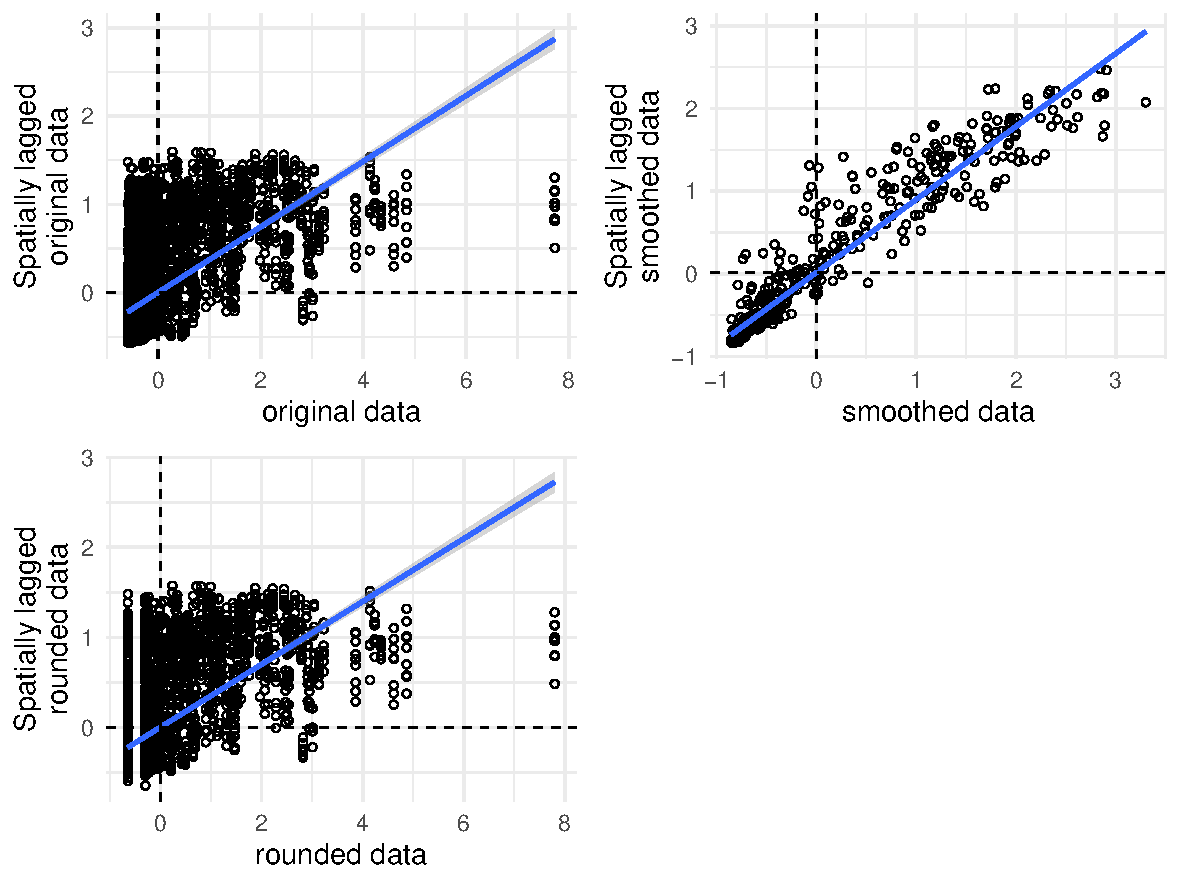
\includegraphics[width=0.8\linewidth]{figures/moran_plot.pdf}
    \caption{Moran's diagrams applied on the number of poor households, with the original data, the data protected by a smoothing method and by a rounding. Be aware that the axes do not have the same scales.}
    \label{fig:moran_plot}
\end{figure}

\section{Local Information Loss} \label{sec:util_LOC}

In sections \ref{sec:util_DD} and \ref{sec:util_SPAT} the metrics discussed were \emph{global}, in the sense of yielding a single aggregate number of information loss for a whole map. Such high-level aggregates often do not capture nuanced distortions, that may nevertheless be relevant to certain data uses \citep{CoxEtAl2011, WooEtAl2009}.
Trivially, if all the distortion occurs in a single small part of the map, the overall information loss may be judged low. But a user specifically interested in that part would nevertheless face a severe inhibition of the maps utility. It is therefore usually a good idea to complement aggregate information loss metrics with \emph{local} measures.

\subsection{Mapping the spatial distribution of error} \label{sec:util_LOC_cellerror}

One way to gain local measures is to `disentangle' global measures and map their individual contributions. In other words, to create a map, where each grid cell displays its individual error value. This allows analyzing the spatial distribution of error. Cell-level measures for the global metrics introduced in \ref{sec:util_DD_hd} are shown in Table \ref{tab:util_cellLVL}.
%\footnote{
    %The cell-level measure pertaining to the Hellinger distance (Eq. \ref{eq:util_hd}) is the squared distance of square roots (SDSR), while the squared error (SE) and absolute error (AE) are the localized parts of the mean squared error (Eq. \ref{eq:util_mse}) and mean absolute error (Eq. \ref{eq:util_mae}) respectively; see \cite{AntalEtAl2017}.}
An example is visualized in Fig. \ref{fig:LErr_maps} (bottom left).

\begin{table}[H]
    \centering
    \begin{tabular}{l c c}
    \hline
    Cell-level measure & Equation & Aggr. measure \\
    \hline
        \rule{0pt}{18pt} Squared dist. of sqr. roots (SDSR) &  $\left(\sqrt{X'_j} - \sqrt{X_j}\right)^2$ & HD \\
        \rule{0pt}{18pt} Squared error (SE) & $\left(X'_j - X_j\right)^2$ & MSE  \\
        \rule{0pt}{18pt} Absolute error (AE) & $\left|X'_j - X_j\right|$ & MAE  \\
        \hline
    \end{tabular}
    \caption{Local information loss metrics based on distributional distances; see also \citet{AntalEtAl2017}.}
    \label{tab:util_cellLVL}
\end{table}

Local information loss measures based on spatial association include the absolute difference in \emph{local} Moran's $\mathcal{I}$ as per Eq.(\ref{localI}) and the absolute difference in local spatial correlation as per Eq.(\ref{eq:dM_i}). Both were introduced in section \ref{sec:util_moran}.

\subsection{Moving window approach / focal error} \label{sec:util_LOC_mw}

A moving window method, also sometimes called \emph{focal statistic}, is a general-purpose grid processing technique, where a value is assigned per grid cell based on the values in that cell's neighborhood. Conceptually, think of a window as a frame of some intermediate size (say, 15 $\times$ 15 cells), symmetrically centered on a single cell, which we call the \emph{focal cell}. The focal cell gets assigned a value that is a function of the $15 \cdot 15 = 225$ cell values currently within the window, but not depending on any values outside of it. \citet{KuhnertEtAl2005} explain how moving window methods may be used for measuring the dissimilarity between grid maps.

In our case, the idea is to assign the focal cell an information loss measure. Specifically, one of the global measures listed above, but computed only based on the cells within the window (therefore `localized'). Straightforward picks are the Hellinger distance (HD), Mean Squared Error (MSE), or Mean Absolute Error (MAE) from section \ref{sec:util_DD_hd}. For example, when using the MAE, the absolute errors are calculated for all, say $225$ cells in the window and their mean is assigned to the focal cell. Subsequently, the window is shifted one cell over and the procedure is repeated.\footnote{
    Moving window methods are typically applied to rectangular grids, either row-wise or column-wise. When the end of a row / column is reached, the window is shifted to the next, until all cells in the grid have been processed.}
The size of the window determines the degree of `localism': the smaller the window, the more local the measure. The moving window approach can therefore implement different levels of `compromise' between global information loss measures (as per \ref{sec:util_DD} and \ref{sec:util_SPAT}) and mapping the cell-level error (as per \ref{sec:util_LOC_cellerror}).

An example is shown in Fig. \ref{fig:LErr_maps} (bottom right). Compared to the cell-level error in Fig. \ref{fig:LErr_maps} (bottom left), the moving window method marks regions of the map where either many cells with some error or a few cells with large error lie together. The parts of the map most impacted should thus be noticeable at a glance.\footnote{
    Note that the size of the region impacted needs to be viewed in conjunction with the size of the error. For instance, in Fig. \ref{fig:LErr_maps} (bottom right), the MAE over 1.5km $\times$ 1.5km chunks is mostly below 5 and in the most afflicted regions %(ca. 1\% of the map) 
    between 5 and 10.}

\begin{figure}
    \centering
    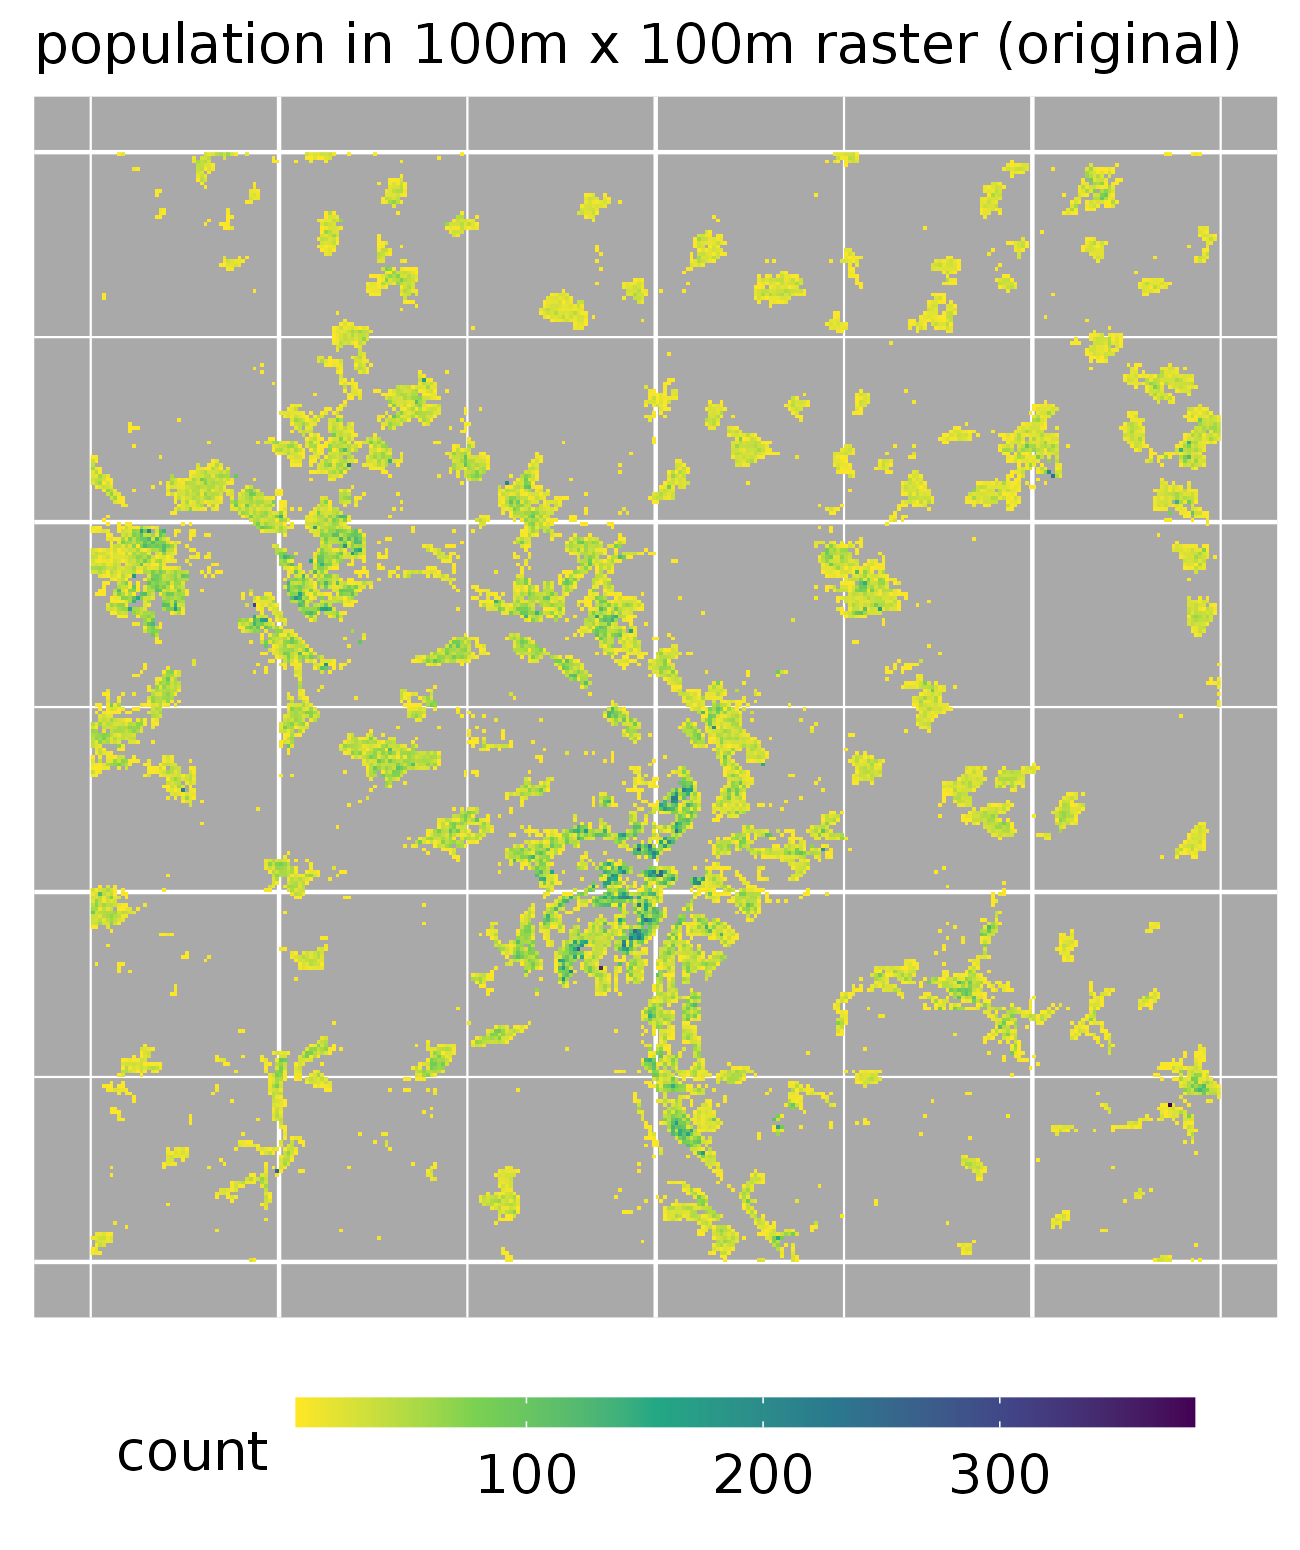
\includegraphics[width=.49\linewidth]{figures/lerr_map_orig.png}
    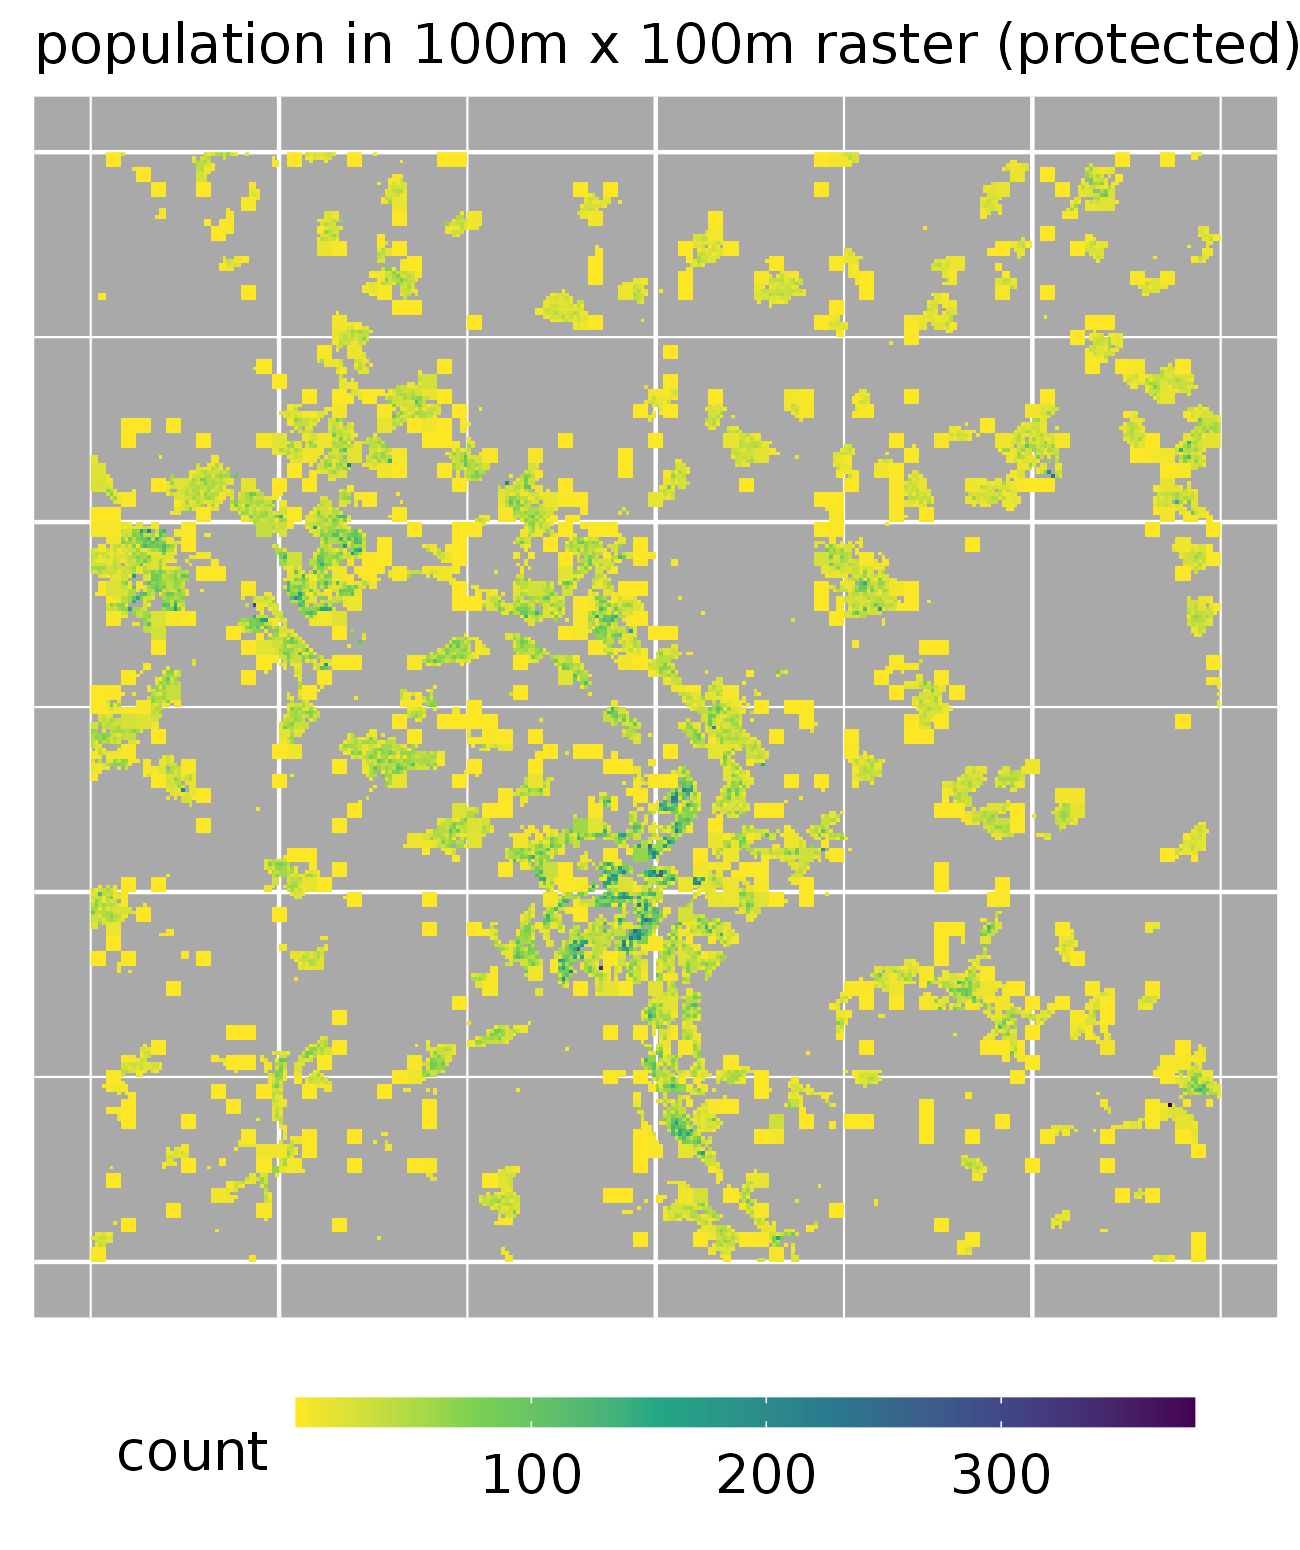
\includegraphics[width=.49\linewidth]{figures/lerr_map_prot.png}
    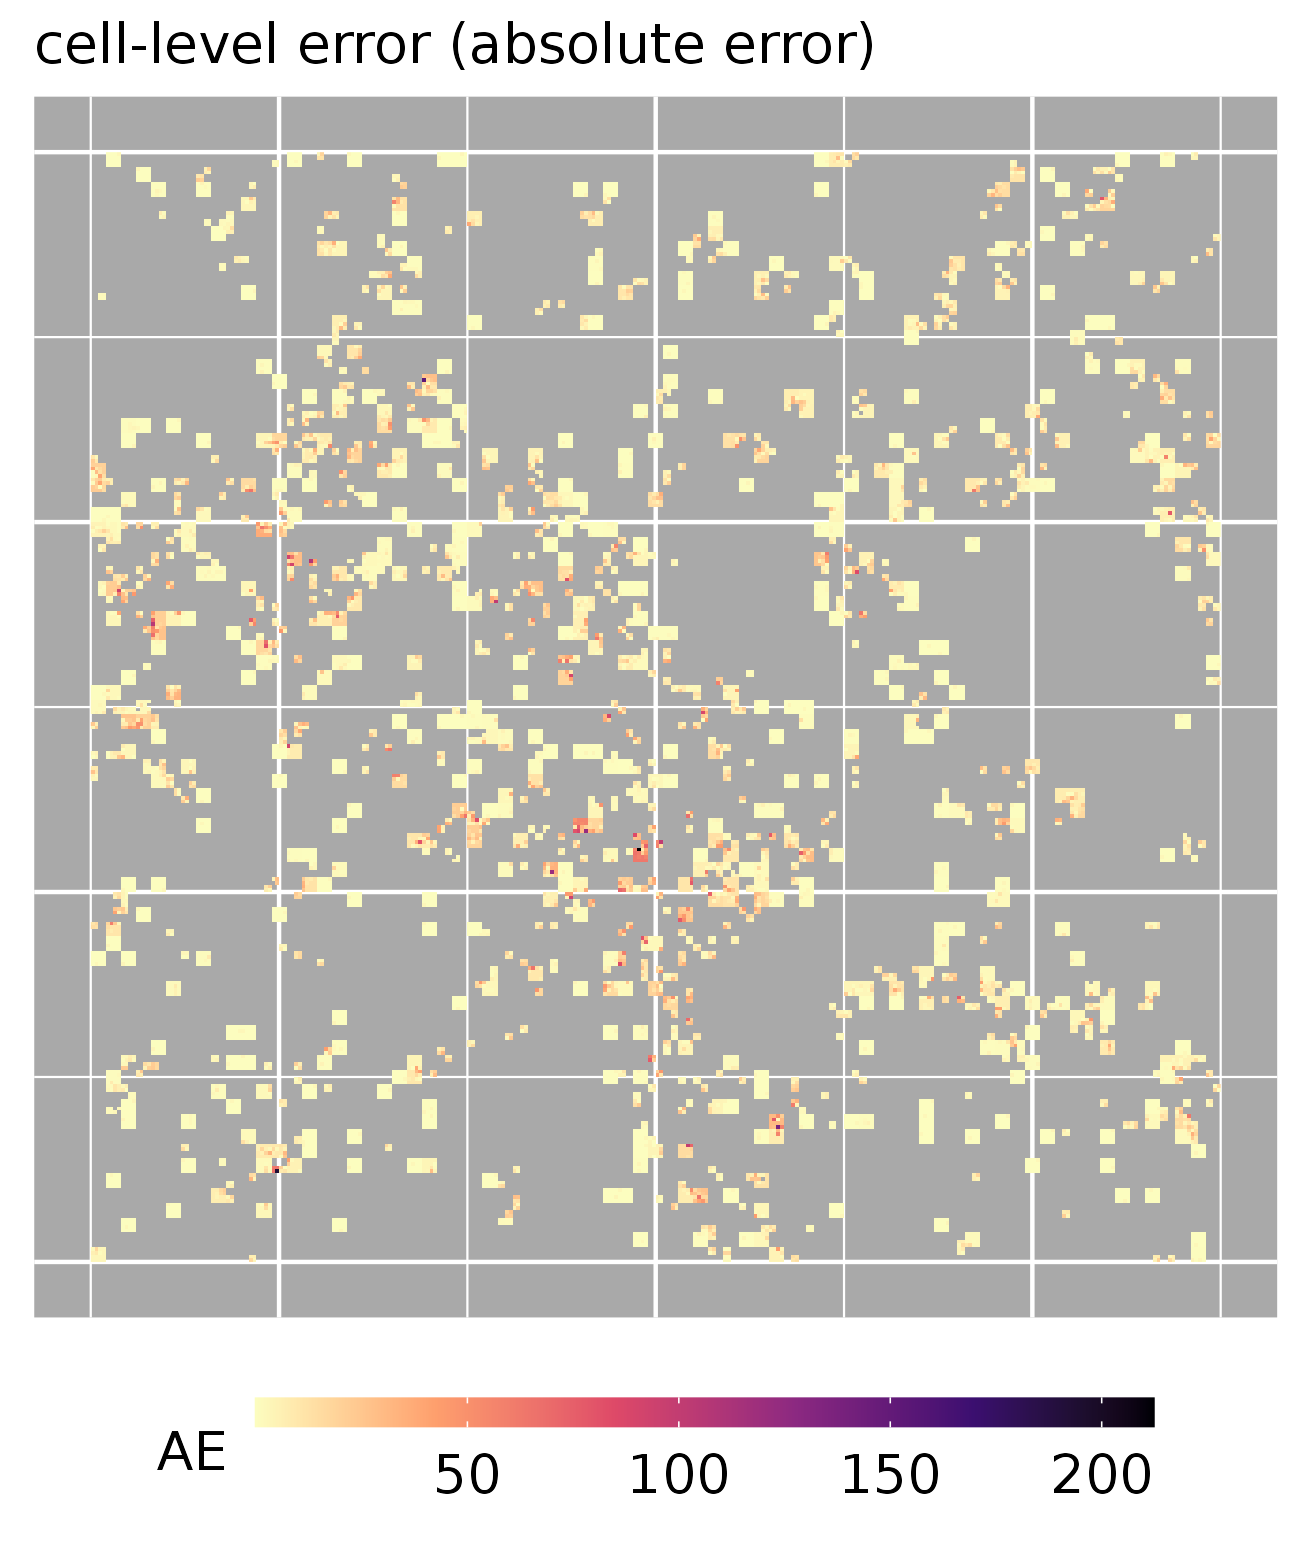
\includegraphics[width=.49\linewidth]{figures/lerr_map_ae.png}
    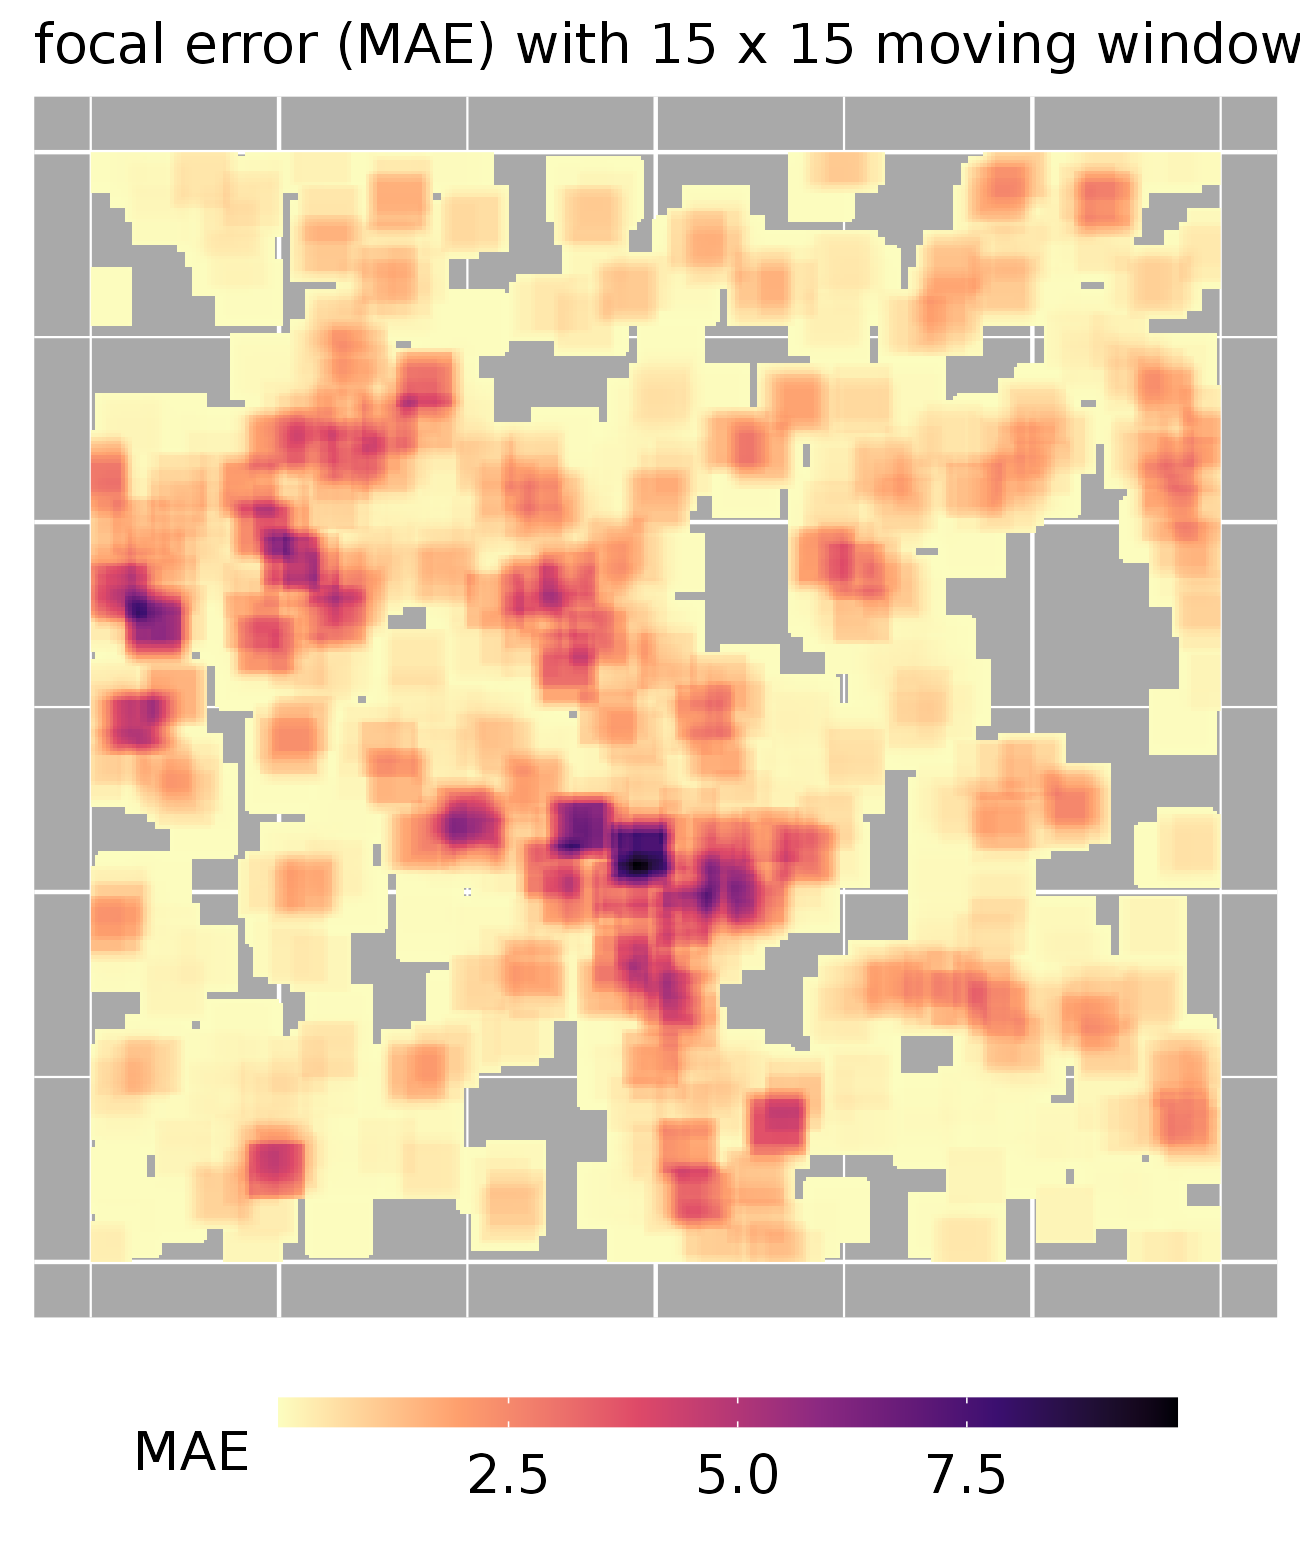
\includegraphics[width=.49\linewidth]{figures/lerr_map_mw_mae.png}
    \caption{Maps of local information loss; top: original map containing small counts (left) and protected map (right) (protection via quadtree algorithm); bottom: cell-level error map with AE measure (left) as per Table \ref{tab:util_cellLVL} and corresponding focal error map of MAE with the moving window method (right) using a window of size 15 $\times$ 15 grid cells.}
    \label{fig:LErr_maps}
\end{figure}


\section{Information Loss Measures and the Modifiable Areal Unit Problem}


Spatial data analysis faces a classical problem known as the Modifiable Areal Unit Problem (MAUP), which denotes two associated sub-problems regarding how spatial data are geographically aggregated:

\begin{itemize}
    \item The zoning effect refers to the sensitivity of results to how the different zones in which the data are grouped are delineated.
    \item The scale effect refers to the geographic precision level of the zoning used: studying a spatial phenomenon at a regional scale may not necessarily lead to the same conclusions as studying it at a municipal scale.
\end{itemize}

\paragraph{Does this problem also concern the data protection stage?}

Actually, any method that influences the delineation of initial geographic areas, primarily by aggregating them, is concerned. Indeed, aggregating two zones to manage a confidentiality issue necessarily generates a zoning problem (the result is sensitive to the chosen zones) and a scale problem (spatial analysis cannot be conducted at the same scale across the entire territory). In this case, information loss measures, especially those based on spatial auto-correlation as the Moran’s $\mathcal{I}$, could be less relevant to compare maps before and after the treatment. Indeed, the comparability of the measures can be lost if the neighbourhoods of the tiles, which the computation of Moran's $\mathcal{I}$ is based on, are modified by the protection process.

Among the methods presented in the chapter~\ref{sec:methods}, only the quadtree method is likely to modify the original level of resolution by aggregating tiles when the confidentiality threshold is not reached (see section~\ref{sec:quadtree}). This modification makes the method sensitive to the zoning effect (since the analysis will be sensitive to the way in which the tiles are aggregated) and to the scale effect (notably because not all tiles will have the same level of resolution). As the Moran’s $\mathcal{I}$ calculation requires to define the neighborhood of each tile, modifying these tiles (by aggregating some of them, for example) modifies their neighborhood (Figure~\ref{fig:queen_neigh}) and, then, makes measurements difficult to compare.

\begin{figure}
    \centering
    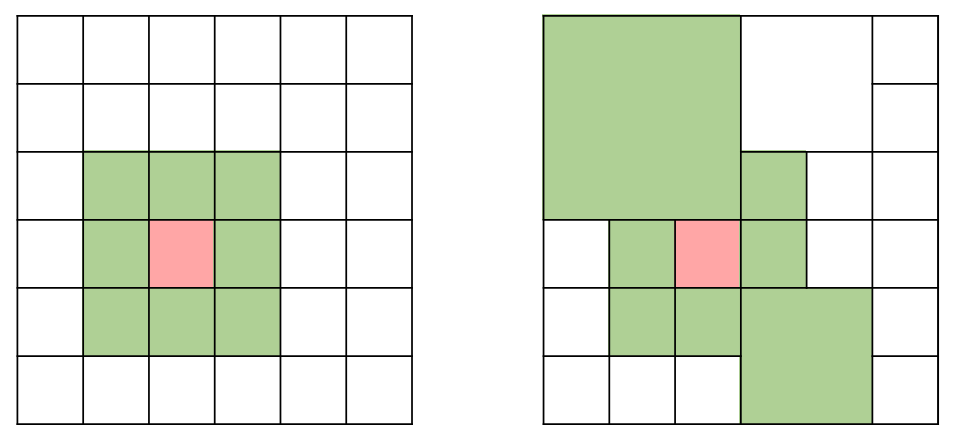
\includegraphics[width=0.75\linewidth]{figures/queen_neighborhood.png}
    \caption{Queen neighborhood (green tiles) of the red tile in the case of a regular grid (left) or an irregular one (right)}
    \label{fig:queen_neigh}
\end{figure}

\paragraph{Another question to ponder is: at what geographic scale should the original and protected maps be compared?}

Users are invited to measure utility (or information loss) at a relevant scale based on the disseminated data and anticipated analyses.

As the information loss cannot be expected to be identical at a global scale (e.g. country level) and at any intermediate or small scale (e.g. region or municipality level), the person in charge of data protection should adapt the scale at which they measure the information loss due to the application of protection methods, depending on the intended uses.

%Let's take the example of the number of households living on the island of La Réunion (France) in 2019. The counts are disseminated in a grid of $200$m $\times$ $200$m tiles. If we compute the Moran's I at the scale of the island, we obtain a Moran's I of $0.521$. But if we calculate Moran's I in each 16km x 16km tile encompassing the island, we obtain a Moran's I ranging from 0.26 to 0.53 depending on the studied area (excluding parts of the island with less than 100 200m tiles).

